\documentclass{beamer}

\usetheme{Madrid}
\usecolortheme{default}
\setbeamerfont{date}{size=\footnotesize}

\hypersetup{
  colorlinks=true,
  urlcolor=blue,
  linkcolor=lime,
  citecolor=magenta
}
\usepackage{xcolor}
\usepackage{tikz}
\usetikzlibrary{arrows.meta, positioning, shapes.geometric}

\newcommand{\cverb}[1]{{\color{purple}{\texttt{#1}}}}

% --- Visual improvements (minimal) ---
% Show a simple section title slide at each new section
\setbeamertemplate{section page}[simple]
\AtBeginSection{\frame{\sectionpage}}

\title[Maintaining a Large Formalisation Project 1]{Maintaining a Large Formalisation Project -- 1}
\subtitle{Part I: Mathematics \& Infrastructure}
\author{Damiano Testa}
\institute[Warwick]{University of Warwick}
\date{Tsinghua University, March 16-20, 2026}

\begin{document}

\begin{frame}
  \titlepage
\end{frame}

\section{Introduction}

% --- Slide: Who Am I ---
\begin{frame}{Who Am I}
I am a mathematician, working on algebraic geometry and number theory.

\bigskip

Since 2020 I have also been interested in formalisation.

\bigskip

My experience with Lean comes from:

\medskip

\begin{itemize}
  \item individual formalisation projects
  \medskip
  \item participating in large collaborations
  \medskip
  \item being a \href{https://github.com/leanprover-community/mathlib}{Mathlib} maintainer
  \medskip
  \item a \href{https://www.renaissancephilanthropy.org/bridging-proof-and-computation-a-verified-leanmacaulay2-interface}{project}, sponsored by AI for Math, to formally verify computations performed by \href{https://macaulay2.com/}{Macaulay2} --- a computer algebra system focusing on commutative algebra and algebraic geometry computations
\end{itemize}
\end{frame}

% --- Separator ---
\begin{frame}{Experience}
\begin{itemize}
  \item \textbf{Formalisation}

  I contributed mostly to the algebraic and order areas of Mathlib.
  \medskip
  \item \textbf{Project-Scale Maintenance and Automation}

  I wrote some linters, as well as some tactics.
  \medskip
  \item \textbf{CI and Infrastructure}

  automated PR summaries, Zulip integration, deprecations.
\end{itemize}
\end{frame}

% --- Next slide from *** ---
\begin{frame}{Recent Projects}
Currently, there are no public major projects that are mostly AI-driven.

\bigskip

Projects using a hybrid approach:

\medskip

\begin{itemize}
  \item the \href{https://terrytao.wordpress.com/2023/03/}{Equational Theory Project}, led by Terry Tao
  \medskip
  \item the \href{https://github.com/thefundamentaltheor3m/Sphere-Packing-Lean}{Sphere Packing Problem in Dimension 8 and 24}, led by Maryna Viazovska and Sidharth Hariharan (\href{https://arxiv.org/abs/2402.06490}{arXiv})
  \medskip
  \item several small formalisations of \href{https://www.erdosproblems.com/}{Erd\H{o}s Problems}
\end{itemize}
\end{frame}

% --- Slide ---
\begin{frame}{If It Works for Humans...}
What I will talk about applies to human-curated repositories.

\bigskip

I will focus on good practices with a view to what I expect would also be useful conventions for AI-generated content.

\bigskip

\begin{block}{Principle}
If something works for humans, maybe AI also benefits from it.
\end{block}
\end{frame}

% --- Slide ---
\begin{frame}{Large Formalisation Projects Involve a Mix of Expertise}
Aspects to keep in mind:

\medskip

\begin{itemize}
  \item Mathematics — planning, development, corrections
  \smallskip
  \item Automation of intermediate task assignments — parallelisability
  \smallskip
  \item Vetting human contributions — code standards, maintainability
  \smallskip
  \item Vetting AI contributions — same as above + guard against exploits
  \smallskip
  \item Final merge decisions — PR quality
  \smallskip
  \item Integration with current project — interoperability
  \smallskip
  \item Re-usability of code-base — API, performance, maintainability
  \smallskip
  \item Automatic detection — linters, naming, docs, guidelines
  \smallskip
  \item CI ensuring main branch stability, caching, tests
  \smallskip
  \item Mathlib bumps — fixes, improvements, refactors
\end{itemize}
\end{frame}

\section{Mathematical Planning}

% --- Mathematics section ---
\begin{frame}{Mathematics}
Most larger formalisation projects start with mathematical planning.

\bigskip

Useful automation:

\medskip

\begin{itemize}
  \item track currently accessible targets
  \medskip
  \item past achievements
  \medskip
  \item partial progress
  \medskip
  \item task assignments
  \medskip
  \item milestones
\end{itemize}
\end{frame}

% --- Slide ---
\begin{frame}{Pre-Requisites}
Some results may be required but out of scope.

\bigskip

For instance, the Feit--Thompson Theorem could be taken with a \cverb{sorry}.

\medskip

\begin{block}{Key Point}
Statements must be formulated \emph{very carefully}.
\end{block}

\begin{itemize}
  \item Misformalisations can poison downstream development.
  \medskip
  \item AI agents may exploit small loopholes.
\end{itemize}
\end{frame}

\section{Blueprints \& Task Distribution}

% --- Slide ---
\begin{frame}{Maths Planning}
Patrick Massot's \href{https://github.com/PatrickMassot/leanblueprint}{blueprint} keeps alignment between LaTeX source and formalisation.

\bigskip

As the formalisation progresses, the initial plan must be:

\medskip

\begin{itemize}
  \item revised
  \smallskip
  \item adapted
  \smallskip
  \item corrected
  \smallskip
  \item expanded
\end{itemize}

\bigskip

Clear partial targets help parallelisation.
\bigskip
\begin{center}
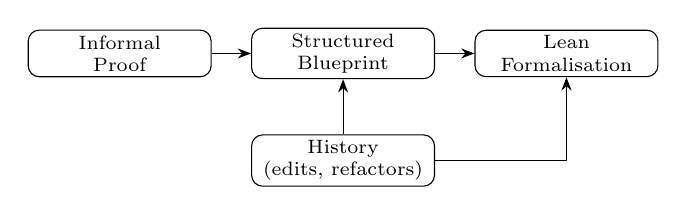
\begin{tikzpicture}[
  >=Stealth,
  node distance=5mm,
  every node/.style={draw, rounded corners, align=center, inner sep=2pt, font=\scriptsize},
  text width=0.18\linewidth,
]
\node (informal) {Informal\\Proof};
\node (blueprint) [right=5mm of informal] {Structured\\Blueprint};
\node (lean) [right=5mm of blueprint] {Lean\\Formalisation};

\draw[->] (informal) -- (blueprint);
\draw[->] (blueprint) -- (lean);

\node (hist) [below=7mm of blueprint] {History\\(edits, refactors)};
\draw[->] (hist) -- (blueprint);
\draw[->] (hist) -| (lean);
\end{tikzpicture}
\end{center}
\end{frame}

% --- Slide ---
\begin{frame}{Distributing Tasks}
\begin{itemize}
  \item Each subproject/lemma/subsection can be assigned independently.
  \medskip
  \item Blueprint ensures all pieces fit together.
  \medskip
  \item Distributing large projects (human + AI) is one of the strengths of formalisation.
\end{itemize}
\end{frame}

\section{Infrastructure \& APIs}

% --- Mathematical infrastructure ---
\begin{frame}{Mathematical Infrastructure: Generating API}
Document and stabilise a small set of canonical interfaces, such as type\cverb{class}es, \cverb{structure}s, \cverb{notation}.

\bigskip

This reduces churn and helps humans and AI.

\bigskip

Enforce good practice, such as
\begin{itemize}
  \item avoid using \cverb{unfold} outside definition files
  \item break off long proofs
  \item generalise whenever possible
\end{itemize}
and so on.
\end{frame}

\section{Quality \& Misformalisations}

% --- Slide: Errors ---
\begin{frame}{Issues and Errors}
Large projects uncover:

\medskip

\begin{itemize}
  \item typos
  \smallskip
  \item omissions
  \smallskip
  \item gaps
  \smallskip
  \item errors
  \smallskip
  \item restructuring needs
\end{itemize}

\bigskip

Fixes may need mathematical experts; small issues may have large ripple effects.

\bigskip

Bigger gaps, may require more serious restructuring.
\end{frame}

% --- Slide: Misformalisations ---
\begin{frame}{Misformalisations}
\begin{columns}[T,totalwidth=\textwidth]
  \begin{column}{0.6\textwidth}
\begin{itemize}
  \item Sometimes definitions differ from intended meaning.
  \medskip
  \item Some informal definitions do not suit dependent type theory.
  \medskip
  \item Need mathematically equivalent but formalisation-friendly formulations.
  \medskip
  \item Fixing an error may lead to proving a lemma that is unsuitable for later development.
\end{itemize}
  \end{column}
  \begin{column}{0.4\textwidth}
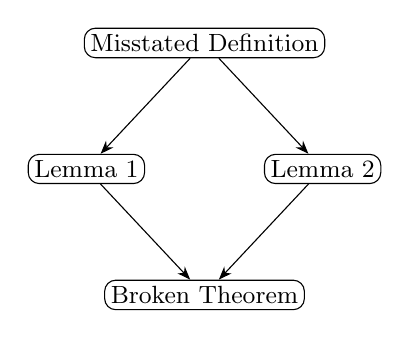
\begin{tikzpicture}[
  >=Stealth,
  every node/.style={draw, rounded corners, align=center, inner sep=2.2pt, font=\small}
]
\node (top) at (0,0) {Misstated Definition};
\node (midL) at (-1.5,-1.6) {Lemma 1};
\node (midR) at ( 1.5,-1.6) {Lemma 2};
\node (bottom) at (0,-3.2) {Broken Theorem};

\draw[->] (top) -- (midL);
\draw[->] (top) -- (midR);
\draw[->] (midL) -- (bottom);
\draw[->] (midR) -- (bottom);
\end{tikzpicture}
  \end{column}
\end{columns}
\end{frame}

% --- Slide: Example ---
\begin{frame}{Example: Correspondence Theorem}

One of the most obvious examples of this is the ubiquitous presence of ``there exists $\ldots$'' statements in informal proofs.

\bigskip

Almost invariably, these purely existential statements hide an explicit construction.

\bigskip

For instance, the \href{https://en.wikipedia.org/wiki/Correspondence_theorem}{Correspondence Theorem} for a group $G$ and a normal subgroup $N$ is stated as the \emph{existence} of a bijection between the subgroups of $G$ containing $N$ and subgroups of the quotient $G / N$.

\bigskip

In practice, it is not the mere \emph{existence} of such a bijection that is important, but rather that we can \emph{explicitly write one down} and we can rely on specific properties of the given bijection.

\bigskip

This means that the ``Correspondence Theorem'' is really a \cverb{def}inition!
\end{frame}

\section{Refactors \& Reusability}

% --- Slide ---
\begin{frame}{Refactors}
For human formalisations, refactors represent a thankless, but essential job.

\bigskip

It is unclear to me if refactors even mean the same for autoformalisation.

\bigskip

I expect that, at some scale, refactoring old code will be more efficient and beneficial than rewriting the whole project from the start.

\bigskip

Refactors should be:

\medskip

\begin{itemize}
  \item standalone PRs
  \smallskip
  \item well-scoped
  \smallskip
  \item accompanied by deprecation shims and migration notes
\end{itemize}
\end{frame}

% --- Slide ---
\begin{frame}{Refactors}

Deprecations may not be needed, but there should be some mechanism for AI to not use the old API.

\bigskip

Changelogs and migration snippets help downstream files update smoothly.

\bigskip

Refactors may be required right after Mathlib bumps or milestone merges.

\bigskip

While this may not apply too much to AI-driven projects, automation for ``common refactors'' is lacking in the ecosystem but highly desired.

\end{frame}

% --- Slide ---
\begin{frame}{Re-Usability of Current Code-Base}
For human-driven projects, reusability is crucial for:

\medskip

\begin{itemize}
  \item long-term maintainability
  \smallskip
  \item enabling broad contributions
  \smallskip
  \item avoid bloating of the code-base
  \smallskip
  \item efficiency and performance
\end{itemize}

\bigskip

Definitions and lemmas should be general when appropriate, avoiding unnecessary specialisation to allow and encourage reuse.
\end{frame}

\section{Maintaining Momentum}

% --- Slide ---
\begin{frame}{Mathlib Bumps}
Mathlib evolves rapidly, but it is good to keep up to date!

\bigskip

Benefits:

\smallskip

\begin{itemize}
  \item bug fixes
  \smallskip
  \item new definitions and lemmas
  \smallskip
  \item improved APIs
  \smallskip
  \item more automation, tactics, diagnostics, performance, $\ldots$
\end{itemize}

\bigskip

Downsides:

\smallskip

\begin{itemize}
  \item break existing proofs
  \smallskip
  \item rename constants
  \smallskip
  \item restructuring of \cverb{import}s
  \smallskip
  \item cause refactors
\end{itemize}
\end{frame}

% --- Slide ---
\begin{frame}{Side Projects}
Useful for exploring:

\medskip

\begin{itemize}
  \item alternative definitions
  \smallskip
  \item rethinking design decisions
  \smallskip
  \item specialized tactics
  \smallskip
  \item computational backends
  \smallskip
  \item refactors
  \smallskip
  \item training specialised agents
\end{itemize}
\end{frame}

% --- Slide ---
\begin{frame}{Fixing Gaps}
Common reasons why a proof resists formalisation:

\medskip

\begin{itemize}
  \item the supplied proof is not detailed enough
  \smallskip
  \item there are some missing hypotheses
  \smallskip
  \item a previous lemma was not proved in enough generality
  \smallskip
  \item there is a mistake in the argument
\end{itemize}

\bigskip

Hopefully this is a rare situation.

\bigskip

When it happens, ``expert'' intervention may be required.

\bigskip

From my perspective, this is a very exciting moment!
\end{frame}

% --- Thanks! ---
\begin{frame}
\begin{center}
  {\huge Thank You!}\\[30pt]
  {\huge Questions?}
\end{center}
\end{frame}

\end{document}
